\documentclass[a4paper]{report}
\usepackage[utf8]{inputenc}
\usepackage[portuguese]{babel}
\usepackage{hyperref}
\usepackage{a4wide}
\hypersetup{pdftitle={UMCarroJá},
pdfauthor={João Teixeira, Emanuel Rodrigues, José Ferreira},
colorlinks=true,
urlcolor=blue,
linkcolor=black}
\usepackage{subcaption}
\usepackage[cache=false]{minted}
\usepackage{listings}
\usepackage{booktabs}
\usepackage{multirow}
\usepackage{appendix}
\usepackage{tikz}
\usepackage{authblk}
\usetikzlibrary{positioning,automata,decorations.markings}

\begin{document}

\title{UMCarroJá\\ 
\large Grupo Nº 48}
\author{João Teixeira (A85504) \and Emanuel Rodrigues (A84776) \and José Ferreira (A83683)}
\date{\today}

\begin{center}
    \begin{minipage}{0.75\linewidth}
        \centering
        
\includegraphics[width=0.4\textwidth]{eng.jpeg}\par\vspace{1cm}
        \vspace{1.5cm}
        \href{https://www.uminho.pt/PT}
        {\color{black}{\scshape\LARGE Universidade do Minho}} \par
        \vspace{1cm}
        {\color{black}{\scshape\Large Programação Orientada a Objetos}} \par
        \vspace{1.5cm}
        \maketitle
    \end{minipage}
\end{center}

\tableofcontents

\pagebreak

\chapter{Introdução}

O objetivo deste projeto é construir um sistema de aluguer de carros,
inspirado no serviço de aluguer de casas \textit{Airbnb}, onde um cliente
pode alugar um carro, onde ele mesmo e o condutor, para fazer a deslocação
que pretende, ou disponibilizar as suas viaturas para alugar. Para a realização
deste projeto vamos aplicar conhecimentos adquiridos nas aulas da U.C. de 
Programação Orientada a Objetos.
Ao longo deste relatório vamos descrever a nossa abordagem a este problema.

\chapter{Classes}\label{chap:api}

\section{Modelo}

\subsection{UMCarroJa}

Esta e a classe onde esta contida toda a informação sobre utilizadores,
carros e alugueres. É também a grande ponte de comunicação com o exterior
do modelo, permitindo assim que não haja interação direta do exterior com
as classes.

\begin{figure}[h]
    \centering
    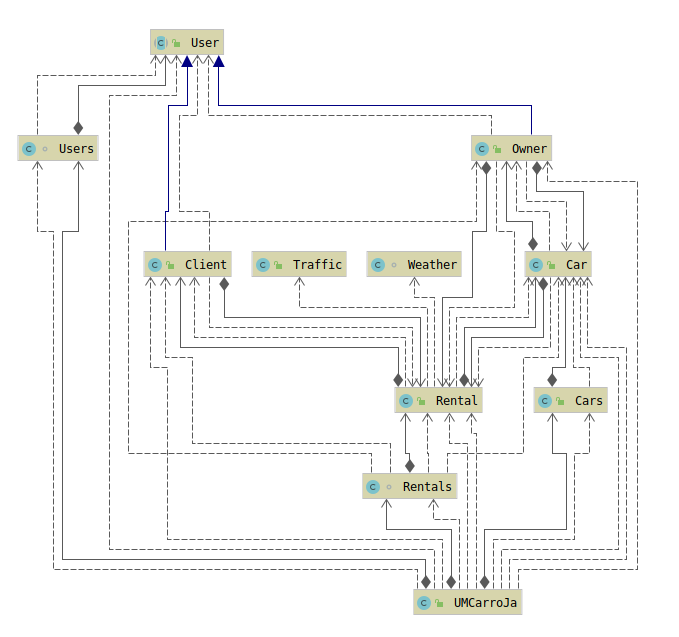
\includegraphics[scale=0.5]{hierarquiaUmCarroJa.png}
    \caption{Hierarquia de Classes do \textbf{UmCarroJa}}\label{fig:hUCJ}
\end{figure}


\subsection{User}

Esta e a classe com a informação contida por qualquer user do sistema,
e métodos comuns tanto aos clientes como aos owners.

\begin{figure}[h]
    \centering
    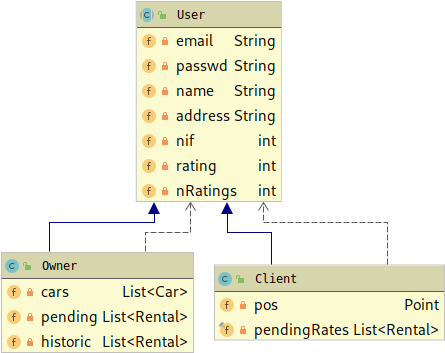
\includegraphics[scale=0.5]{hierarquiaUser.png}
    \caption{Hierarquia de Classes do \textbf{User}}
\end{figure}

\subsection{Client}

Esta classe é referente ao user que pode criar alugueres, contendo
esta um Ponto, correspondente à posição em que se encontra e alugueres
que ainda não foram avaliados.

\subsection{Owner}

Esta classe é relativa ao utilizador que tem os seus carros para aluguer,
e este tem informação sobre os carros que possui e também os alugueres
que ainda não avaliou.

\subsection{Users}

Esta classe contem a informação de todos os utilizadores do sistema.

\subsection{Car}

Esta classe representa uma viatura, onde tem todas as suas informações,
desde autonomia, quem é o seu proprietário, marca e matricula.

\subsection{Cars}

Esta classe trata de guardar todos os carros existentes no sistema, bem
como procurar carros conforme as condições dadas para efetuar um aluguer.

\subsection{Rental}

Esta classe contem todos os métodos para gerar e tratar um aluguer.

\subsection{Rentals}

Esta classe guarda a informacao relativa a todos os alugueres efetuados
no sistema.

\subsection{Parser}

Esta classe tem como objetivo a leitura do ficheiro de logs e transformacao
em infomacao utilizavel pelo programa.

\section{View}

\subsection{Menu}

Esta classe representa os vários Menus e as relações entre eles. Para permitir
conhecer o caminho percorrido até ao menu que se está a observar, esta classe
contém uma stack com os menus percorridos.

\subsection{Table}

Esta classe representa uma Tabela com um generic type parameter. Para tal
apenas precisa de uma lista de Labels para as colunas, outra para as linhas e
os dados sobre a forma de uma Lista de Listas.
O resultado final é uma tabela em que cada coluna tem o tamanho mínimo possível.

\subsection{ViewModel}

Esta Package contem um conjunto de classes que permitem a transferência de argumentos
entre a View e o Controller de forma mais legível. Por exemplo, a classe RegisterCar
contém todos os parâmetros necessários para registar um novo carro e uma instância desta
é passada da View para o Controller a fim de o adicionar aos carros.

\section{Controller}

Cria a ponte entre o View e o Model. Assim, o Controller é o único que conhece a view e o
Model, sendo que tanto a View como o Model apenas conhecem o Controller.

\section{Utils}

\subsection{Point}

Esta classe contém as coordenadas de um ponto num plano, assim como métodos sobre estes.
Por exemplo, um método para para calculara a distância entre dois pontos.

\subsection{StringBetter}

Esta classe contém métodos para converter uma string para quando for
impressa no ecrã tenha várias propriedades. Tais como terem cor
específica, estarem sublinhadas e pedir uma palavra passe ao utilizador sem mostrar os caracteres escritos.

\section{Exceptions}

Esta Package contém todas as classes de exceções utilizadas ao longo do projeto.

\chapter{Arquitetura e Solução do Projeto}

\section{Modelo}

No modelo, todos os pedidos entram pela classe UmCarroJa como visivel na hieraquia de classes desta\ref{fig:hUCJ}, a salvo excecoes, como alguns 
gets sobre classes deste. Daqui sao chamados todos os metodos das outras
classes necessarios a realizar os pedidos.

\chapter{Introducao de novos tipos de Viaturas}

Neste momento, e a luz do ficheiro de logs fornecido, todos os carros sao
tratados de igual maneira, pelo que a diferenciacao entre os diversos tipos
de veiculos e feita atraves de um \textit{enum}. 

\chapter{Testes}

\section{Manutenção de Artigos}

Para testar a Manutenção de Artigos foram criados dois programas em Python.
O primeiro gera input em que as instruções dadas são válidas mas aleatórias.
O segundo gera um conjunto de instruções que é válido e é possível testar se estão
a ser bem interpretadas.
\begin{itemize} 
    \item Adiciona N produtos (passados como argumento), em que o nome é igual ao id do
        produto e o preço é igual a 0.
    \item Altera o nome de todos os produtos para 10 vezes o seu id.
    \item Altera o preço de todos os produtos para ser igual ao seu id.
\end{itemize}
Assim, para ver se o resultado é o esperado basta verificar se para um dado id
este tem preço igual a id e tem um nome igual a 10 vezes o id.

\section{Cliente de Vendas}

Para testar o Cliente de Vendas foram criados dois programas em Python que
seguem a mesma lógica dos criados para a Manutenção de Artigos.
O primeiro gera input em que as instruções dadas são válidas mas aleatórias.
O segundo gera um conjunto de instruções que é válido e é possível testar se estão
a ser bem interpretadas.
\begin{itemize} 
    \item Acede a todos os ids.
    \item Adiciona ao stock 100 artigos de cada artigo.
    \item Remove do stock 10 artigos de cada artigo.
\end{itemize}
Assim, para verificar se o resultado é o esperado podemos confirmar se para um dado
id o stock disponível é igual a 90.
Na mesma veia, se vários Clientes de Vendas correrem em concorrência, para validar
os resultados é possível verificar se a fórmula \textit{stock / 90 = N}, sendo o stock o stock
disponível para um dado artigo e N o número de clientes de vendas que foram corridos
em concorrência, é verdade.

\chapter{Conclusão}

Para concluir, conseguimos cumprir todos os requisitos propostos criando no processo um
sistema de gestão de stocks capaz de utilizar uma arquitetura \textit{Cliente, Servidor}
que suporta várias centenas de clientes.
Como trabalho futuro, gostaríamos de melhorar a relação entre o Manutenção de Artigos e
o Cliente de Vendas.

\end{document}
